This chapter shows some of the basec algorithms and implementations required to solve problems that include graphs.

\section{Depth First Search (DFS)}

The DFS algorithm is a recursive algorithm that visits all the nodes of a graph. It is used to find connected components, topological sorting, and to find bridges and articulation points. The algorithm is as follows:

\begin{algorithm}
\caption{Depth First Search (DFS)}
\label{alg:dfs}
\begin{algorithmic}[1]
\Procedure{DFS}{$G$}
\State $visited \gets \emptyset$
\State $time \gets 0$
\State $parent \gets \emptyset$
\State $low \gets \emptyset$
\State $disc \gets \emptyset$
\State $AP \gets \emptyset$
\State $bridge \gets \emptyset$
\ForAll{$v \in V$}
\State $visited[v] \gets false$
\State $parent[v] \gets -1$
\State $low[v] \gets \infty$
\State $disc[v] \gets \infty$
\EndFor
\ForAll{$v \in V$}
\If{$visited[v] = false$}
\State DFSUtil($G$, $v$, $visited$, $time$, $parent$, $low$, $disc$, $AP$, $bridge$)
\EndIf
\EndFor
\EndProcedure
\Procedure{DFSUtil}{$G$, $v$, $visited$, $time$, $parent$, $low$, $disc$, $AP$, $bridge$}
\State $visited[v] \gets true$
\State $disc[v] \gets time$
\State $low[v] \gets time$
\State $time \gets time + 1$
\State $children \gets 0$
\ForAll{$u \in Adj(v)$}
\If{$visited[u] = false$}
\State $parent[u] \gets v$
\State $children \gets children + 1$
\State DFSUtil($G$, $u$, $visited$, $time$, $parent$, $low$, $disc$, $AP$, $bridge$)
\State $low[v] \gets min(low[v], low[u])$
\If{$parent[v] = -1$ and $children > 1$}
\State $AP[v] \gets true$
\EndIf
\If{$parent[v] != -1$ and $low[u] \geq disc[v]$}
\State $AP[v] \gets true$
\EndIf
\If{$low[u] > disc[v]$}
\State $bridge[v][u] \gets true$
\EndIf
\Else
\State $low[v] \gets min(low[v], disc[u])$
\EndIf
\EndFor
\EndProcedure
\end{algorithmic}
\end{algorithm}

The implementation can be done as follows:

\lstinputlisting{../Graphs/DFS.cpp}

An application of this algorithm in order to find the shorteast path between two nodes can be done as follows:


\lstinputlisting{../Graphs/DFS-application.cpp}

\section{Breadth First Search (BFS)}

The BFS algorithm is a non-recursive algorithm that visits all the nodes of a graph. It is used to find connected components, topological sorting, and to find bridges and articulation points, to better understand it, a propagating fire can be imagined. The algorithm is as follows:

\begin{algorithm}
\caption{Breadth First Search (BFS)}
\label{alg:bfs}
\begin{algorithmic}[1]
\Procedure{BFS}{$G$}
\State $visited \gets \emptyset$
\State $time \gets 0$
\State $parent \gets \emptyset$
\State $low \gets \emptyset$
\State $disc \gets \emptyset$
\State $AP \gets \emptyset$
\State $bridge \gets \emptyset$
\ForAll{$v \in V$}
\State $visited[v] \gets false$
\State $parent[v] \gets -1$
\State $low[v] \gets \infty$
\State $disc[v] \gets \infty$
\EndFor
\ForAll{$v \in V$}
\If{$visited[v] = false$}
\State BFSUtil($G$, $v$, $visited$, $time$, $parent$, $low$, $disc$, $AP$, $bridge$)
\EndIf
\EndFor
\EndProcedure
\Procedure{BFSUtil}{$G$, $v$, $visited$, $time$, $parent$, $low$, $disc$, $AP$, $bridge$}
\State $visited[v] \gets true$
\State $disc[v] \gets time$
\State $low[v] \gets time$
\State $time \gets time + 1$
\State $children \gets 0$
\ForAll{$u \in Adj(v)$}
\If{$visited[u] = false$}
\State $parent[u] \gets v$
\State $children \gets children + 1$
\State BFSUtil($G$, $u$, $visited$, $time$, $parent$, $low$, $disc$, $AP$, $bridge$)
\State $low[v] \gets min(low[v], low[u])$
\If{$parent[v] = -1$ and $children > 1$}
\State $AP[v] \gets true$
\EndIf
\If{$parent[v] != -1$ and $low[u] \geq disc[v]$}
\State $AP[v] \gets true$
\EndIf
\If{$low[u] > disc[v]$}
\State $bridge[v][u] \gets true$
\EndIf
\Else
\State $low[v] \gets min(low[v], disc[u])$
\EndIf
\EndFor
\EndProcedure
\end{algorithmic}
\end{algorithm}

The implementation can be done as follows:

%\inputminted{c++}{Graphs/BFS.cpp}
\lstinputlisting{../Graphs/BFS.cpp}

%\VerbatimInput{Graphs/BFS.cpp}

\section{Finding Bridges and Articulation Points}

The following algorithms are used to find bridges and articulation points in a graph. The implementation of these algorithms is done using DFS and BFS. This algoithms are based on Tarjan's algorithm.

Tarjan's algorithm is an algorithm that is used to find bridges and articulation points in a graph. The algorithm is as follows:

\begin{algorithm}
\caption{Tarjan's Algorithm}
\label{alg:tarjan}
\begin{algorithmic}[1]
\Procedure{Tarjan}{$G$}
\State $visited \gets \emptyset$
\State $time \gets 0$
\State $parent \gets \emptyset$
\State $low \gets \emptyset$
\State $disc \gets \emptyset$
\State $AP \gets \emptyset$
\State $bridge \gets \emptyset$
\ForAll{$v \in V$}
\State $visited[v] \gets false$
\State $parent[v] \gets -1$
\State $low[v] \gets \infty$
\State $disc[v] \gets \infty$
\EndFor
\ForAll{$v \in V$}
\If{$visited[v] = false$}
\State TarjanUtil($G$, $v$, $visited$, $time$, $parent$, $low$, $disc$, $AP$, $bridge$)
\EndIf
\EndFor
\EndProcedure
\Procedure{TarjanUtil}{$G$, $v$, $visited$, $time$, $parent$, $low$, $disc$, $AP$, $bridge$}
\State $visited[v] \gets true$
\State $disc[v] \gets time$
\State $low[v] \gets time$
\State $time \gets time + 1$
\State $children \gets 0$
\ForAll{$u \in Adj(v)$}
\If{$visited[u] = false$}
\State $parent[u] \gets v$
\State $children \gets children + 1$
\State TarjanUtil($G$, $u$, $visited$, $time$, $parent$, $low$, $disc$, $AP$, $bridge$)
\State $low[v] \gets min(low[v], low[u])$
\If{$parent[v] = -1$ and $children > 1$}
\State $AP[v] \gets true$
\EndIf
\If{$parent[v] != -1$ and $low[u] \geq disc[v]$}
\State $AP[v] \gets true$
\EndIf
\If{$low[u] > disc[v]$}
\State $bridge[v][u] \gets true$
\EndIf
\Else
\State $low[v] \gets min(low[v], disc[u])$
\EndIf
\EndFor
\EndProcedure
\end{algorithmic}
\end{algorithm}

\lstinputlisting{../Graphs/Tarjan_y_BlockCutTree.cpp}

\subsection{Bridges}

A bridge is an edge that if it is removed, the graph will be divided into two or more components. The implementation is:

\lstinputlisting{../Graphs/FindBridges.cpp}


\subsection{Articulation Points}

An articulation point is a node that if it is removed, the graph will be divided into two or more components. The implementation is:

\lstinputlisting{../Graphs/FindArticulationPoints.cpp}

\section{Flows}

The flow is a concept that is used in many algorithms, it is used to find the maximum flow that could go through a system of nodes.

\subsection{Dinic}

The Dinic algorithm is a useful algorithm to find the maximum flow that could go through a system of nodes. The implementation of this algorithm is:

\lstinputlisting{../Graphs/Dinic.cpp}

This implementation is done in order to do the Dinic algorithm for a graph with a large number of nodes.

This algorithm is based on the idea of the BFS algorithm, it is used to find the shortest path between two nodes, in this case, the shortest path between the source and the sink. The algorithm is as follows:

\begin{algorithm}
\caption{Dinic}
\label{alg:dinic}
\begin{algorithmic}[1]
\Procedure{Dinic}{$G$}
\State $visited \gets \emptyset$
\State $time \gets 0$
\State $parent \gets \emptyset$
\State $low \gets \emptyset$
\State $disc \gets \emptyset$
\State $AP \gets \emptyset$
\State $bridge \gets \emptyset$
\ForAll{$v \in V$}
\State $visited[v] \gets false$
\State $parent[v] \gets -1$
\State $low[v] \gets \infty$
\State $disc[v] \gets \infty$
\EndFor
\ForAll{$v \in V$}
\If{$visited[v] = false$}
\State DinicUtil($G$, $v$, $visited$, $time$, $parent$, $low$, $disc$, $AP$, $bridge$)
\EndIf
\EndFor
\EndProcedure
\Procedure{DinicUtil}{$G$, $v$, $visited$, $time$, $parent$, $low$, $disc$, $AP$, $bridge$}
\State $visited[v] \gets true$
\State $disc[v] \gets time$
\State $low[v] \gets time$
\State $time \gets time + 1$
\State $children \gets 0$
\ForAll{$u \in Adj(v)$}
\If{$visited[u] = false$}
\State $parent[u] \gets v$
\State $children \gets children + 1$
\State DinicUtil($G$, $u$, $visited$, $time$, $parent$, $low$, $disc$, $AP$, $bridge$)
\State $low[v] \gets min(low[v], low[u])$
\If{$parent[v] = -1$ and $children > 1$}
\State $AP[v] \gets true$
\EndIf
\If{$parent[v] != -1$ and $low[u] \geq disc[v]$}
\State $AP[v] \gets true$
\EndIf
\If{$low[u] > disc[v]$}
\State $bridge[v][u] \gets true$
\EndIf
\Else
\State $low[v] \gets min(low[v], disc[u])$
\EndIf
\EndFor
\EndProcedure
\end{algorithmic}
\end{algorithm}

\subsection{Ford Fulkerson}

The Ford Fulkerson algorithm is a useful algorithm to find the maximum flow that could go through a system of nodes. The implementation of this algorithm is:

\lstinputlisting{../Graphs/FordFulkerson.cpp}

In order to better understand the adjecency matrix in the code Figure \ref{fig:ford_fulkerson} shows the graph that is used in the code.

\begin{figure}[h]
\centering
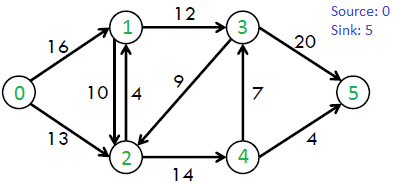
\includegraphics[width=0.35\textwidth]{../Figures/ford_fulkerson11.png}
\caption{Ford Fulkerson}
\label{fig:ford_fulkerson}
\end{figure}
